\capitulo{3}{Conceptos teóricos}


\section{CRUD}
En el ámbito de la programación un CRUD es un acrónimo que agrupa las cuatro operaciones básicas que son necesarias para gestionar y manejar datos en una aplicación:

\begin{center}
  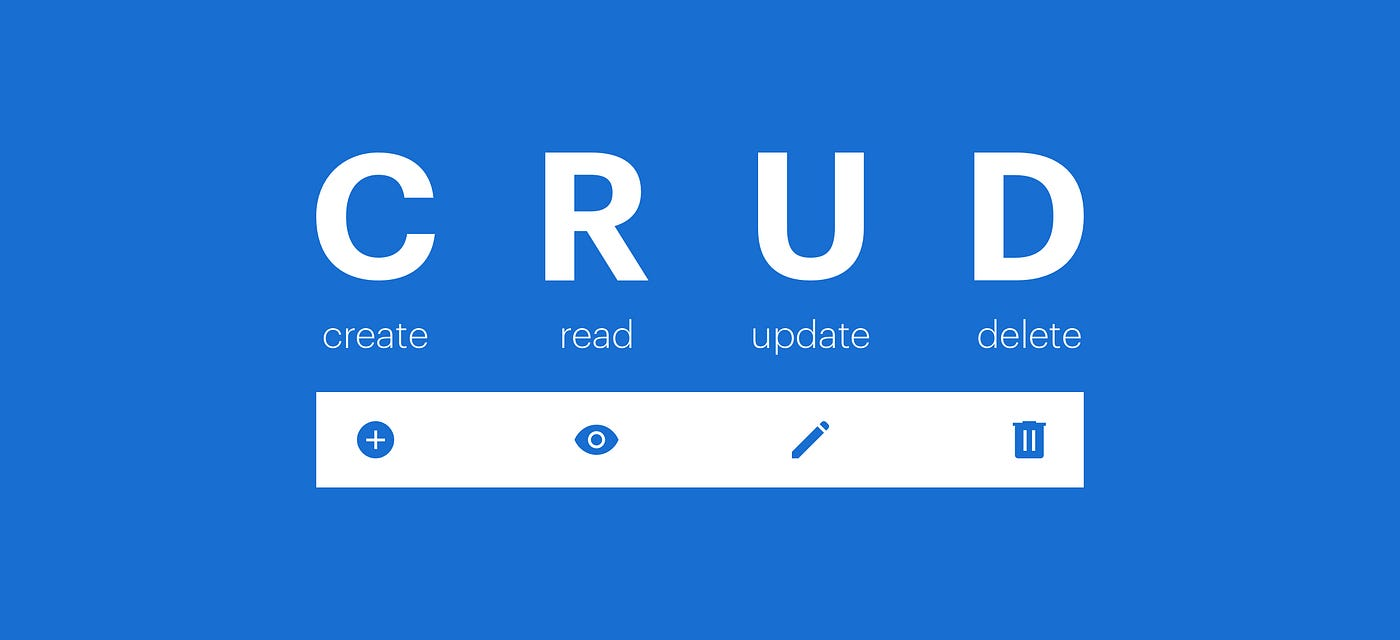
\includegraphics[width=0.6\textwidth]{img/crud-logo.jpg}\\
  \small Definición de CRUD
\end{center}

\subsection{Create (Crear)}
Consiste en la inserción de nuevos registros o nuevos datos en una base de datos. Por ejemplo, dar de alta un usuario o meter un partido nuevo.

\subsection{Read (Leer)}
Consiste en la consulta de los datos ya existentes en la base de datos. Permite mostrar listados con datos, detalles o resultados de búsquedas sin modificar la información original. Por ejemplo, consultar la lista de partidos guardados.

\subsection{Update (Actualizar)}
Consiste en hacer modificaciones de registros o datos ya existentes. Se utiliza para corregir, completar o cambiar valores. Por ejemplo, actualizar la fecha de un partido guardado.

\subsection{Delete (Eliminar)}
Consiste en borrar registros o datos que ya no son necesarios. Implica borrar los datos de la base de datos. Por ejemplo, borrar un partido que finalmente no se jugará.


Cada operación de un CRUD se puede traducir como sentencias a nivel de base de datos.
Por ejemplo INSERT para Create, SELECT para Read, UPDATE para Update, DELETE para Delete.
 


\section{API}
El concepto de API (Application Programming Interfaces) o Interfaz de Programación de Aplicaciones engloba las funciones, herramientas, reglas y endpoints que nos permiten tener una comunicación directa para poder extraer información o datos, además de funcionalidades interesantes.

Las APIs son muy necesarias para proyectos como este que tienen un CRUD. Las APIs exponen puntos de entrada (endpoints) que permiten ejecutar operaciones CRUD de forma controlada desde puntos externos a la API (en este caso desde la interfaz de la página web). El funcionamiento consiste en asignar a cada endpoint una operacion CRUD de forma clara. Por ejemplo POST /usuarios para Create, GET /usuarios/{id} para Read, PUT /usuarios/{id} para Update, DELETE /usuarios/{id} para Delete.

Las APIs pueden ser abiertas, que son APIs de código abierto que permiten obtener datos gratuitos. Pueden ser internas o propias, creadas por un usuario (como en este caso, creadas por mí) Pueden ser de pago, que necesitan que un usuario pague una suscripción para poder sacar datos y usar los endpoints o funcionalidades.


\section{Endpoints}
Los endpoints son los puntos de acceso que se definen dentro de una API y que permiten la comunicación entre aplicaciones. Cada uno de los endpoints corresponden a una URL en específico y tienen asociada una determinada operación como puede ser la obtención de datos, creación de algún recurso o herramienta o actualización de la información. Estos endpoints actúan como puertas de acceso, recibiendo solicitudes del cliente y devolviendo respuestas. Lo más normal es combinarlos con métodos HTTP como son GET, POST, PUT y DELETE para así identificar la acción que se desea realizar.


\section{Métodos HTTP}
Los métodos http son las acciones que van a indicar al servidor que tipo de operacion se quiere realizar sobre un determinado recurso cuando se crea una solicitud a través de una API. Los métodos más comunes y los que se manejan en la aplicación creada son:
\subsection{GET}
Solicita datos sin modificarlos.

\subsection{POST}
Crea un nuevo dato o un nuevo recurso.

\subsection{PUT}
Actualiza un dato o recurso que ya existe.

\subsection{DELETE}
Elimina un dato o recurso que ya existe.

Existen otros métodos como el OPTIONS o el PATCH que sirven para consultar capacidades de un endpoint
y para hacer actualizaciones parciales respectivamente.


\section{Front-End}
El front-end es una de las capas de la aplicación web, en concreto la capa con la que interactúa de forma directa el usuario. En este caso está construido con tecnologías como HTML, CSS y TypeScript porque he usado Angular. Se encarga elegir que datos se presentan y como se presentan (colores, estilos, tipos de letra, etc.).

\section{Back-End}
El back-end es la otra capa de la aplicación web, que es la parte que es invisible para el usuario final y se ocupa de llevar toda la lógica, manejo de datos y la seguridad de los datos. Está implementado en este caso en .NET y conecta con base de datos (en este caso MySQL en HeidiSQL) en las que almacena, recupera y actualiza información. Esta parte de la web expone APIs y endpoints que despues consumirá el front-end para mostrar la información.

\section{Full-Stack}
El full-stack es la combinación de las dos capas de la aplicación (front-end y back-end), coordinando la lógica con la representación de los datos. Además, engloba la gestión de las bases de datos y la integración de algunos servicios externos.


\begin{center}
  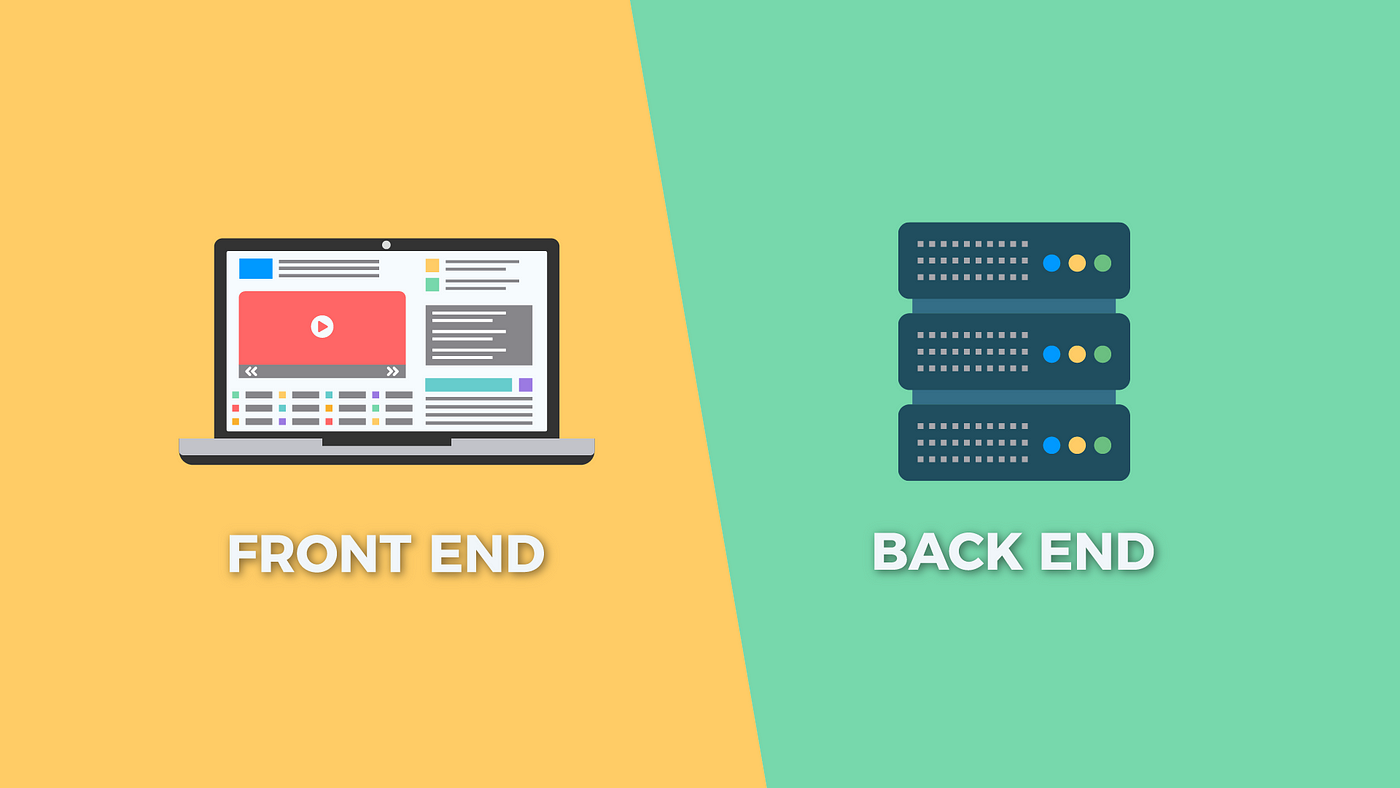
\includegraphics[width=0.7\textwidth]{img/front-back.png}\\
  \small Visual Front vs Back
\end{center}